% =====================================================================
%  Supplementary Material
%  A Training-Free Quantum-Walk Scanner for Cryptic Allosteric Sites
%  Global Quantum + AI Challenge 2026 - Cleveland Clinic - Phase I
%  (Optional supplementary, <= 3 pages, per Submission Guidelines 4.4)
% =====================================================================
\documentclass[10pt,a4paper]{article}
\usepackage[T1]{fontenc}
\usepackage[utf8]{inputenc}
\usepackage{mathptmx}
\usepackage{microtype}
\usepackage{graphicx}
\usepackage[margin=2.2cm,top=2.0cm,bottom=2.0cm]{geometry}
\usepackage{amsmath,amssymb}
\usepackage{booktabs}
\usepackage{tabularx}
\usepackage{array}
\usepackage{xcolor,colortbl}
\usepackage{titlesec}
\usepackage[hidelinks]{hyperref}
\usepackage{caption}
\definecolor{v5tint}{RGB}{234,230,247}   % light purple = delivered model
\newcolumntype{V}{>{\columncolor{v5tint}\centering\arraybackslash}p{1.15cm}}
\setlength{\parskip}{0.3em}\setlength{\parindent}{0pt}
\titlespacing*{\section}{0pt}{0.8em}{0.3em}
\titleformat{\section}{\normalfont\large\bfseries}{\thesection.}{0.6em}{}
\captionsetup{font=small,labelfont=bf,skip=3pt}
\newcommand{\B}[1]{\textbf{#1}}

\begin{document}

\begin{center}
  {\large\bfseries Supplementary Material}\\[3pt]
  {\small A Training-Free Quantum-Walk Scanner for Cryptic Allosteric Sites\\
   Global Quantum + AI Challenge 2026 $\cdot$ Cleveland Clinic Enterprise Challenge $\cdot$ Phase~I}
\end{center}
\vspace{0.4em}

% =====================================================================
\section{Delivered-model evaluation}

The delivered ranking is the coherent directed current on the chiral Laplacian generator, scored by the
distance-deconfounded $z(j)$. All numbers below come from exact classical simulation on the
13-protein set (10 calibration + 3 blind validation); ground truth is the $4$\,\AA\ heavy-atom rule.
Entry 1IE4 is undefined because all its labelled residues fall inside the active-site-plus-first-neighbour
exclusion, leaving zero candidate positives --- an honest structural guard, not a failure.

Table~\ref{tab:literal} reports the challenge-literal test (Guidelines \S4.1): one-sided Mann--Whitney
$U$ of $z$(distal positives) against (T1) random surface background and (T2) non-functional fpocket
residues, as rank-biserial effect size $r_{\mathrm{rb}}$ and Holm-corrected $p$ across targets.
Table~\ref{tab:auc} reports blind ranking quality as distance-matched AUROC of the delivered current
against the trivial $-$distance geometric baseline (the confound level). Results are shown in full,
not filtered.

\begin{table}[h]
\centering
\caption{Challenge-literal significance of the delivered (distance-corrected) $z(j)$. Bold = Holm
$p<0.05$. $r_{\mathrm{rb}}\!\in\![-1,1]$: $+1$ = positives rank above the negative set, $0$ = no
difference. 2RD5 has a single distal positive (unstable).}
\label{tab:literal}
\small
\begin{tabularx}{\textwidth}{@{}lcc rr rr cc@{}}
\toprule
 & & & \multicolumn{2}{c}{\textbf{T1 vs background}} & \multicolumn{2}{c}{\textbf{T2 vs pockets}} & \multicolumn{2}{c}{\textbf{hit}}\\
\cmidrule(lr){4-5}\cmidrule(lr){6-7}\cmidrule(lr){8-9}
\textbf{Target} & \textbf{$N$} & \textbf{$n_{+}$} & $r_{\mathrm{rb}}$ & $p_{\mathrm{Holm}}$ & $r_{\mathrm{rb}}$ & $p_{\mathrm{Holm}}$ & @5 & @10\\
\midrule
\multicolumn{9}{@{}l}{\emph{Calibration (10 proteins)}}\\
1IE4  & 120 & 0  & ---   & ---   & ---   & ---   & --- & ---\\
4OFG  & 142 & 23 & 0.36  & 0.057 & 0.51  & \B{0.002} & 0 & 1\\
4B1F  & 255 & 8  & 0.45  & 0.137 & 0.50  & 0.085 & 1 & 1\\
5J5S  & 258 & 18 & 0.42  & \B{0.029} & 0.34 & 0.087 & 1 & 1\\
2RD5  & 282 & 1  & 1.00  & 0.102 & 1.00  & 0.087 & 1 & 1\\
3MWB  & 305 & 10 & $-$0.01 & 1.000 & $-$0.29 & 1.000 & 0 & 0\\
4KZT  & 432 & 14 & $-$0.26 & 1.000 & $-$0.09 & 1.000 & 0 & 0\\
1M8P  & 573 & 18 & $-$0.39 & 1.000 & $-$0.37 & 1.000 & 0 & 0\\
1YV3  & 703 & 10 & $-$0.21 & 1.000 & $-$0.30 & 1.000 & 0 & 0\\
2Y0P  & 847 & 18 & $-$0.02 & 1.000 & $-$0.01 & 1.000 & 0 & 0\\
\midrule
\multicolumn{9}{@{}l}{\emph{Blind validation (3 targets)}}\\
KRAS G12C      & 169 & 10 & 0.14 & 1.000 & 0.40 & 0.150 & 0 & 1\\
BCR-ABL1       & 451 & 17 & \B{0.60} & \B{$<$0.001} & \B{0.60} & \B{$<$0.001} & 1 & 1\\
Cardiac myosin & 954 & 9  & 0.13 & 1.000 & 0.06 & 1.000 & 0 & 0\\
\bottomrule
\end{tabularx}
\end{table}

\begin{table}[h]
\centering
\caption{Blind ranking quality across the 13-protein benchmark: distance-matched AUROC of the
\emph{delivered} coherent directed current (V5, shaded) against the single-time directed flux (V3, $J$)
and the classical comparators --- average mixing $\hat M$, communicability $e^{A}$, degree, and the
$-$distance geometric baseline. \B{Bold} marks the delivered model above chance ($>0.5$); ``---'' = no
distal positive after filtering. Training targets are ranked by length $N$; the three blind validation
targets follow the rule. Classical readouts collapse to $\approx$chance once the geometric confound is
controlled.}
\label{tab:auc}
\footnotesize
\setlength{\tabcolsep}{5pt}\renewcommand{\arraystretch}{1.12}
\begin{tabular}{@{}llr r V r r r r@{}}
\toprule
\textbf{Protein} & \textbf{Split} & \textbf{$N$} & \textbf{$J$ (V3)} & \textbf{current (V5)} & \textbf{$\hat M$} & \textbf{$e^{A}$} & \textbf{degree} & \textbf{$-$dist}\\
\midrule
1IE4  & train & 120 & ---  & ---        & ---  & ---  & ---  & ---\\
4OFG  & train & 142 & 0.50 & \B{0.76}   & 0.50 & 0.50 & 0.54 & 0.50\\
4B1F  & train & 255 & 0.35 & \B{0.70}   & 0.44 & 0.32 & 0.23 & 0.74\\
5J5S  & train & 258 & 0.46 & \B{0.68}   & 0.61 & 0.53 & 0.48 & 0.84\\
2RD5  & train & 282 & 0.65 & \B{1.00}   & 0.57 & 0.13 & 0.21 & 0.86\\
3MWB  & train & 305 & 0.72 & 0.43       & 0.71 & 0.33 & 0.51 & 0.14\\
4KZT  & train & 432 & 0.54 & 0.43       & 0.34 & 0.43 & 0.66 & 0.63\\
1M8P  & train & 573 & 0.82 & 0.30       & 0.48 & 0.43 & 0.47 & 0.09\\
1YV3  & train & 703 & 0.40 & 0.37       & 0.47 & 0.69 & 0.37 & 0.90\\
2Y0P  & train & 847 & 0.30 & 0.47       & 0.39 & 0.42 & 0.42 & 0.32\\
\midrule
KRAS G12C      & val & 169 & 0.60 & \B{0.67} & 0.34 & 0.33 & 0.33 & 0.54\\
BCR-ABL1       & val & 451 & 0.62 & \B{0.77} & 0.42 & 0.27 & 0.66 & 0.73\\
Cardiac myosin & val & 954 & 0.56 & \B{0.54} & 0.53 & 0.45 & 0.37 & 0.64\\
\midrule
\textbf{Mean (12)} & & & 0.54 & \cellcolor{v5tint}\B{0.59} & 0.48 & 0.40 & 0.44 & 0.58\\
\textbf{Mean (val)} & & & 0.59 & \cellcolor{v5tint}\B{0.66} & 0.43 & 0.35 & 0.45 & 0.64\\
\bottomrule
\end{tabular}
\end{table}

\B{Reading the result.} On the flagship blind target BCR-ABL1 the delivered score separates the distal
allosteric residues from \emph{both} negative sets with large effect ($r_{\mathrm{rb}}\!\approx\!0.6$)
and survives Holm correction across all targets ($p<0.001$), and its distance-matched AUROC ($0.77$)
beats the geometric baseline. Signal is present but weaker or absent on other targets, reported
honestly; the directed current exists only through quantum coherence (Fig.~\ref{fig:budget}), so it is
a genuinely quantum discriminator rather than a re-expression of geometry.

% =====================================================================
\section{Coherence budget and resource scaling}

Figures generated by \texttt{notebooks/coherence\_feasibility.ipynb} in the public repository, using the
current best model on BCR-ABL1.

\begin{figure}[h]
\centering
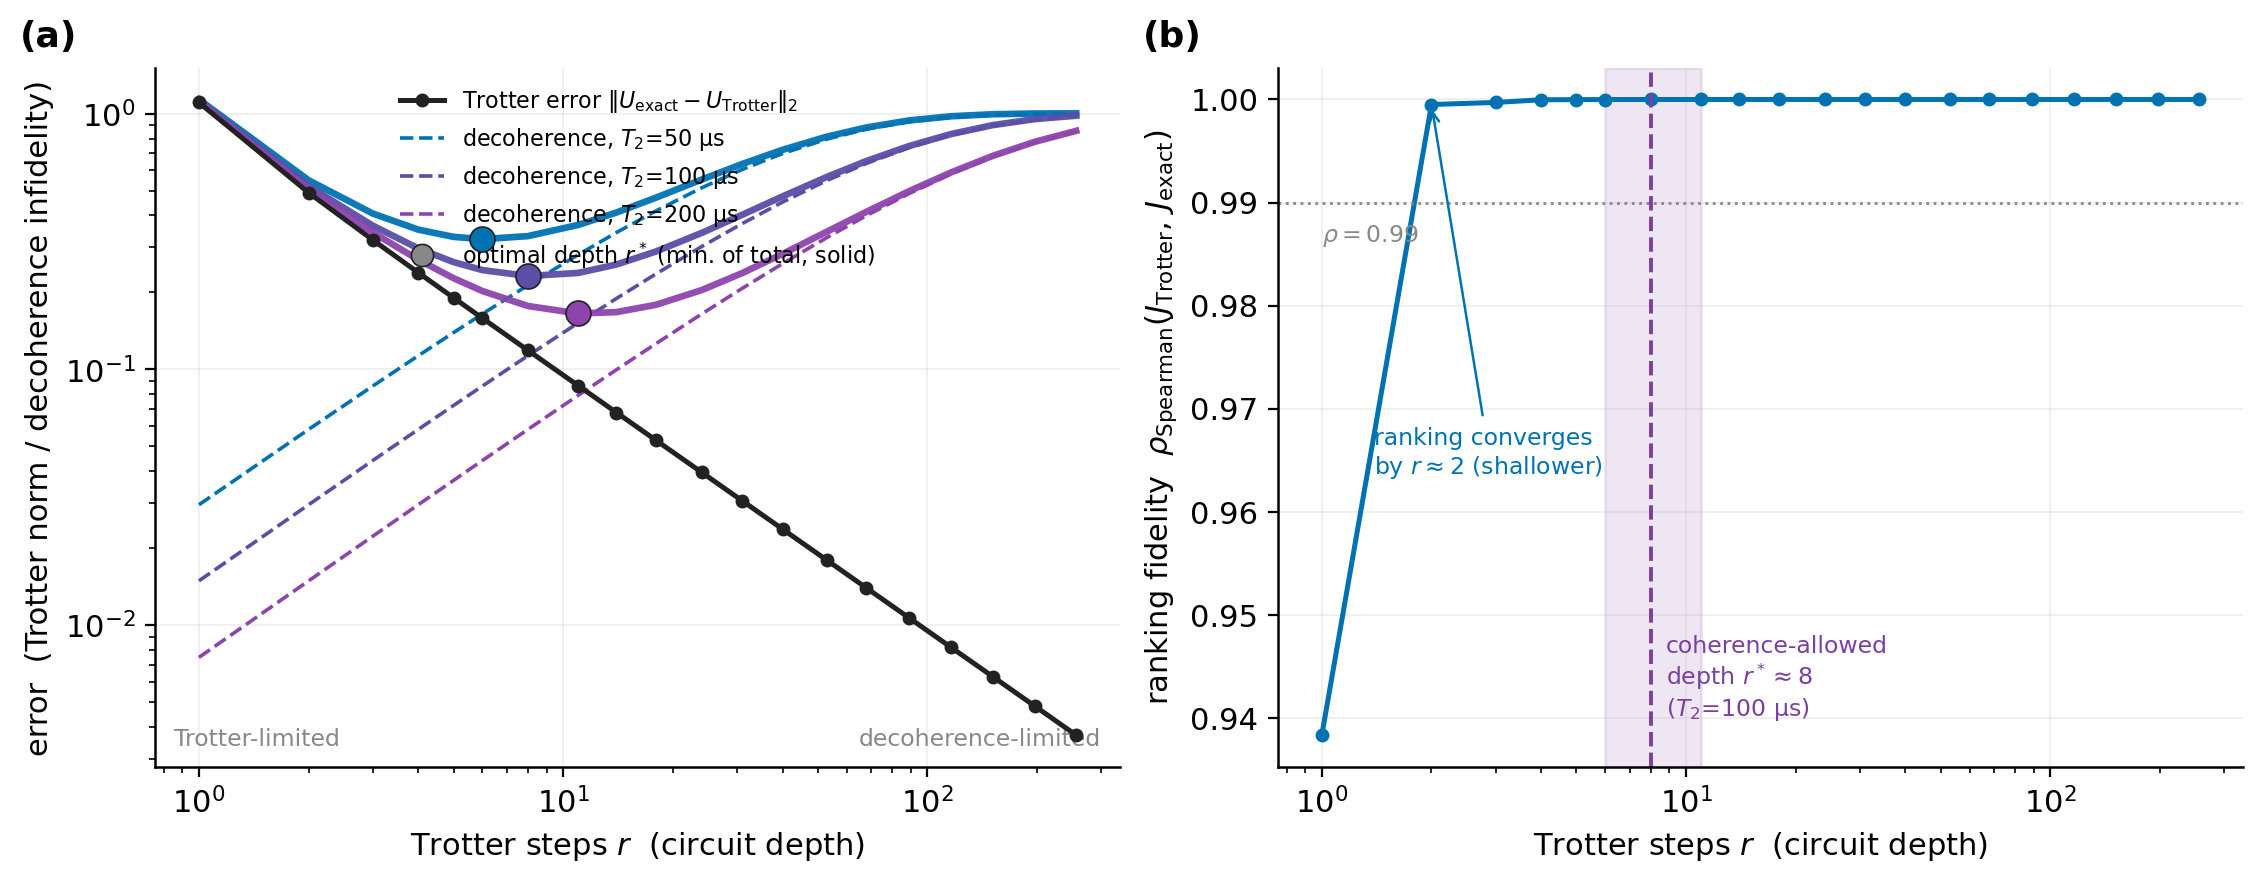
\includegraphics[width=0.92\textwidth]{figs/fig4_coherence_budget.png}
\caption{\textbf{Coherence-time budget.} (a) Systematic Trotter error falls with circuit depth $r$
while decoherence infidelity rises; their sum is U-shaped with an optimal depth $r^{*}\propto\sqrt{T_2}$.
(b) The ranking converges at a depth well inside the coherence-allowed $r^{*}$, so a hardware
demonstration sits comfortably within the coherence budget.}
\label{fig:budget}
\end{figure}

\begin{figure}[h]
\centering
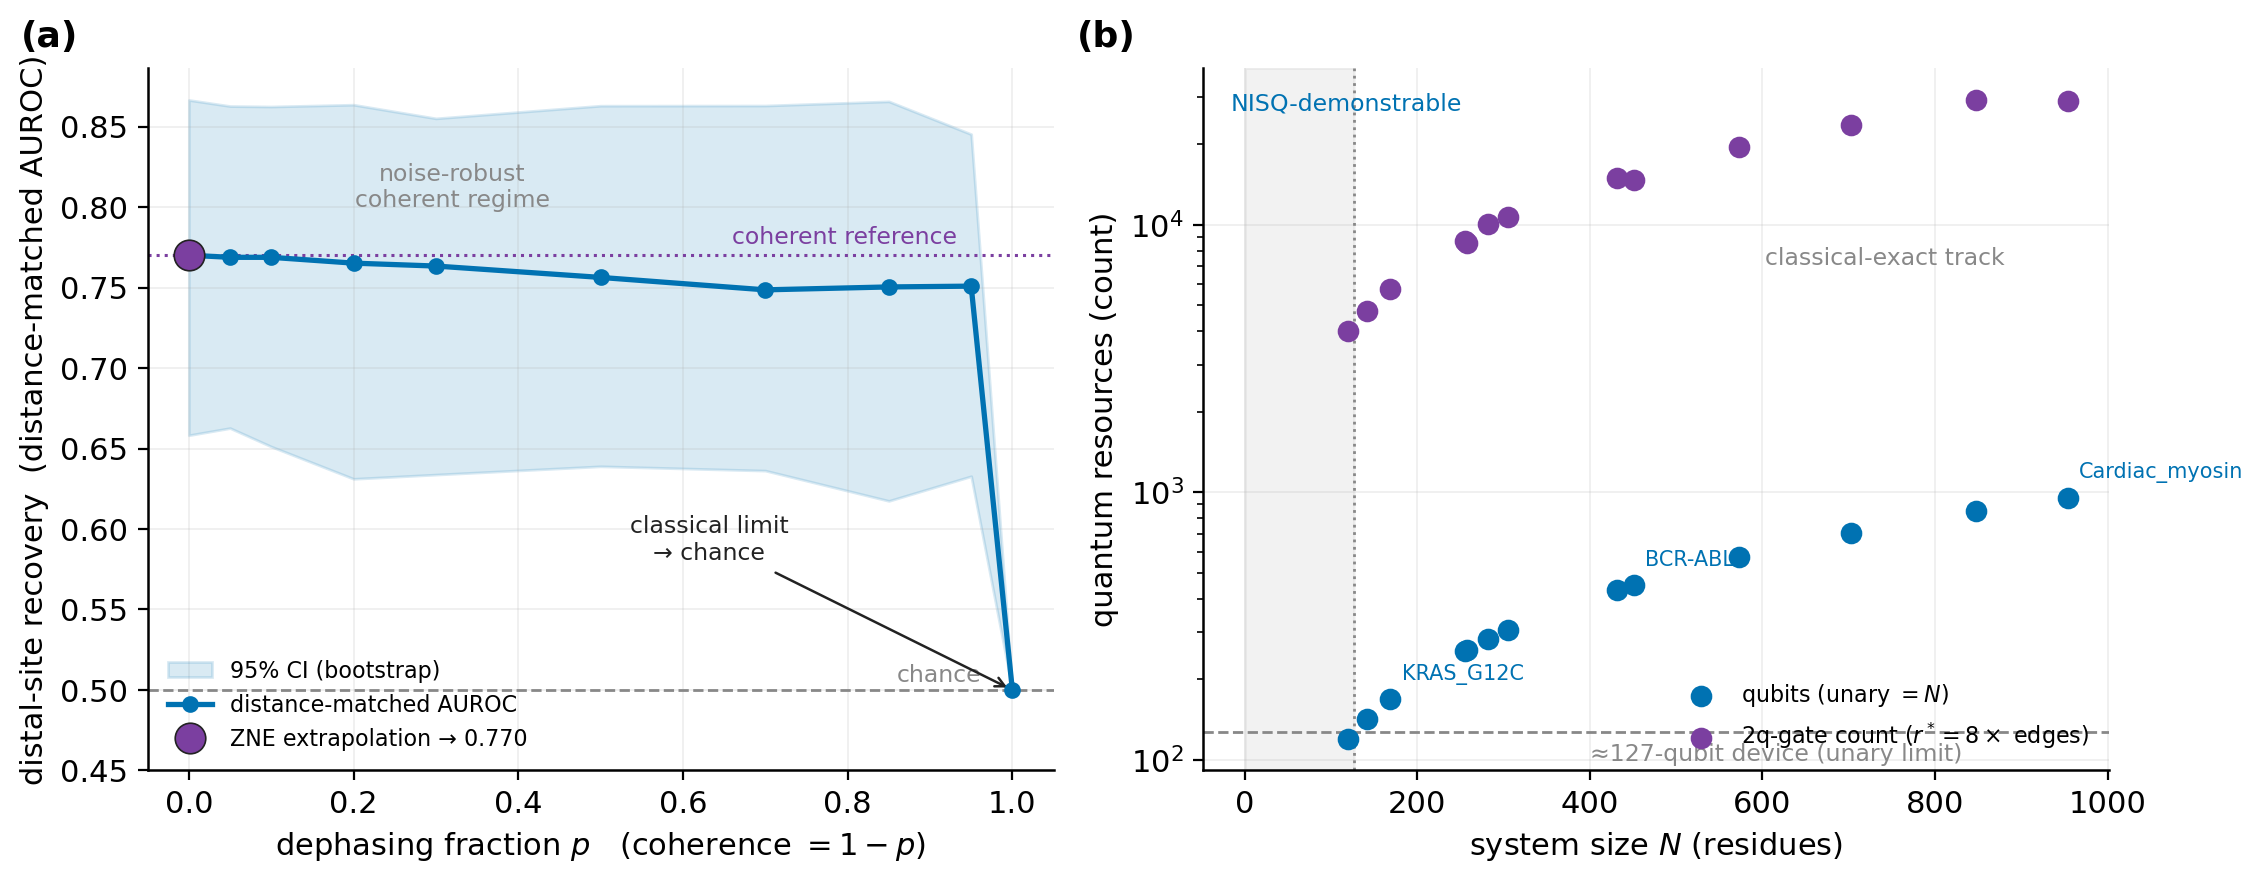
\includegraphics[width=0.92\textwidth]{figs/fig5_noise_resource.png}
\caption{\textbf{Noise resilience and NISQ resource scaling.} (a) Distal-site recovery vs the dephasing
fraction $p$: robust across the coherent regime and collapsing to chance at the fully classical limit
($p{=}1$), evidence that the signal is coherence-borne; a zero-noise extrapolation recovers the
coherent value. (b) Unary qubit count equals residue count and two-qubit gate count scales with
contact edges: small targets are demonstrable on near-term devices, larger ones are delivered on the
exact classical track.}
\label{fig:resource}
\end{figure}

\end{document}
